\documentclass[12pt]{article}
\usepackage{amsmath,amssymb}
\usepackage{booktabs}
\usepackage{natbib}
\usepackage{hyperref}
\usepackage{microtype}
\usepackage{xcolor}
\usepackage{mdframed}
\usepackage{enumitem}
\usepackage{graphicx}
\usepackage{caption}
\usepackage{geometry}
\geometry{margin=1in}
\usepackage{xr}
\externaldocument{hrf}

% Referee comment box
\newmdenv[
  linecolor=gray!50,
  backgroundcolor=gray!8,
  innerleftmargin=10pt,
  innerrightmargin=10pt,
  innertopmargin=8pt,
  innerbottommargin=8pt,
  skipabove=10pt,
  skipbelow=4pt
]{refbox}

\newcommand{\tcr}{\textcolor{red}}
\newcommand{\tcm}{\textcolor{magenta}}
\newcommand{\tcg}{\textcolor{green}}

\newcommand{\comment}[1]{\begin{refbox}\textit{#1}\end{refbox}}
\newcommand{\response}{\medskip\noindent\textbf{Response.}\ }

\title{Response to Report by Referee 1\\[6pt]
  \large ``The Hedged Random Forest''\\
  \normalsize Journal of Financial Econometrics --- JFEC-2025-167}
\author{E.\ Beck \and D.\ Kozbur \and M.\ Wolf}
\date{}

\begin{document}
\maketitle
\thispagestyle{empty}

We thank the referee for the careful reading and constructive suggestions.
The report has led to meaningful improvements in the paper.
Below we address each point in turn.
All section, equation, and table references are to the revised manuscript.

% ============================================================
\section*{Main Comments}
% ============================================================

% -----------------------------------------------------------
\subsection*{Comment 1}
% -----------------------------------------------------------

\comment{Why not carry out estimation on a second sample using standard OLS
with constraints on the weights, which is also a standard approach
(Timmermann, 2006)?  Ridge would require to tune a parameter, but this
could be done by AIC, though ad hoc.  Of course, this is a different
estimator, but a reader may want to understand the distinction and whether
one approach is better than the other.}

\response
We have implemented a second-sample benchmark in the spirit of
\citet{timmermann:2006}.
The approach splits the training data in half: the random forest is trained
on the first half, and the tree-level weights are estimated on the second
half (which the trees have never seen).

A standard OLS estimator on the second sample is not viable here because the
number of trees ($p = 500$) exceeds the second-sample size ($n/2$) in some settings,
making the system underdetermined.
Ridge regression with a sum-to-one constraint handles the high-dimensional
regime gracefully; we select the penalty parameter $\lambda$ by AIC.
We refer to this estimator as \textit{2-Step Ridge}.

The empirical results are reported in Figure~\ref{fig:2step-ridge} below
(green boxplots). 2-Step Ridge is dominated by HRF at every
training-set size we consider, not merely in an isolated instability
region: even away from $n \approx 2p = 1000$, its mean RMSE ratio
relative to HRF sits around 0.87--0.93 (that is, HRF's RMSE is
7--13\% lower). This gap becomes much more severe as the training-set
size approaches twice the number of trees ($n \approx 2p = 1000$),
because the second-stage regression is then estimated from about as
many observations as there are trees to weight; this causes its RMSE to
spike relative to HRF by more than an order of magnitude at $n = 1000$.

The persistent gap away from $n = 1000$ is plausibly explained by the
sample-splitting procedure itself: the random forest underlying 2-Step
Ridge is trained on only the first half of the training set ($n/2$
observations), whereas HRF's forest uses the full sample ($n$
observations). 2-Step Ridge therefore starts from a structurally weaker
forest at every training-set size, quite apart from the instability
associated with estimating $w$ near $n \approx 2p$. This, together with
the instability documented above, illustrates the benefit of estimating
the covariance matrix $\Sigma$ via nonlinear shrinkage on the full
training sample, as HRF does, rather than resorting to sample
splitting.

Because this instability is so pronounced, including 2-Step Ridge in the
manuscript's Figure~\ref{fig:win} would force an axis scale that obscures
the comparison of HRF with the other, better-behaved benchmarks (WRF,
CRF, Ridge, and HRF-MinVar), which all lie within a narrow band around a
ratio of one. We have therefore decided to keep 2-Step Ridge out of the
manuscript itself and report it here instead, where it can be discussed
on its own terms.

\medskip
\begin{center}
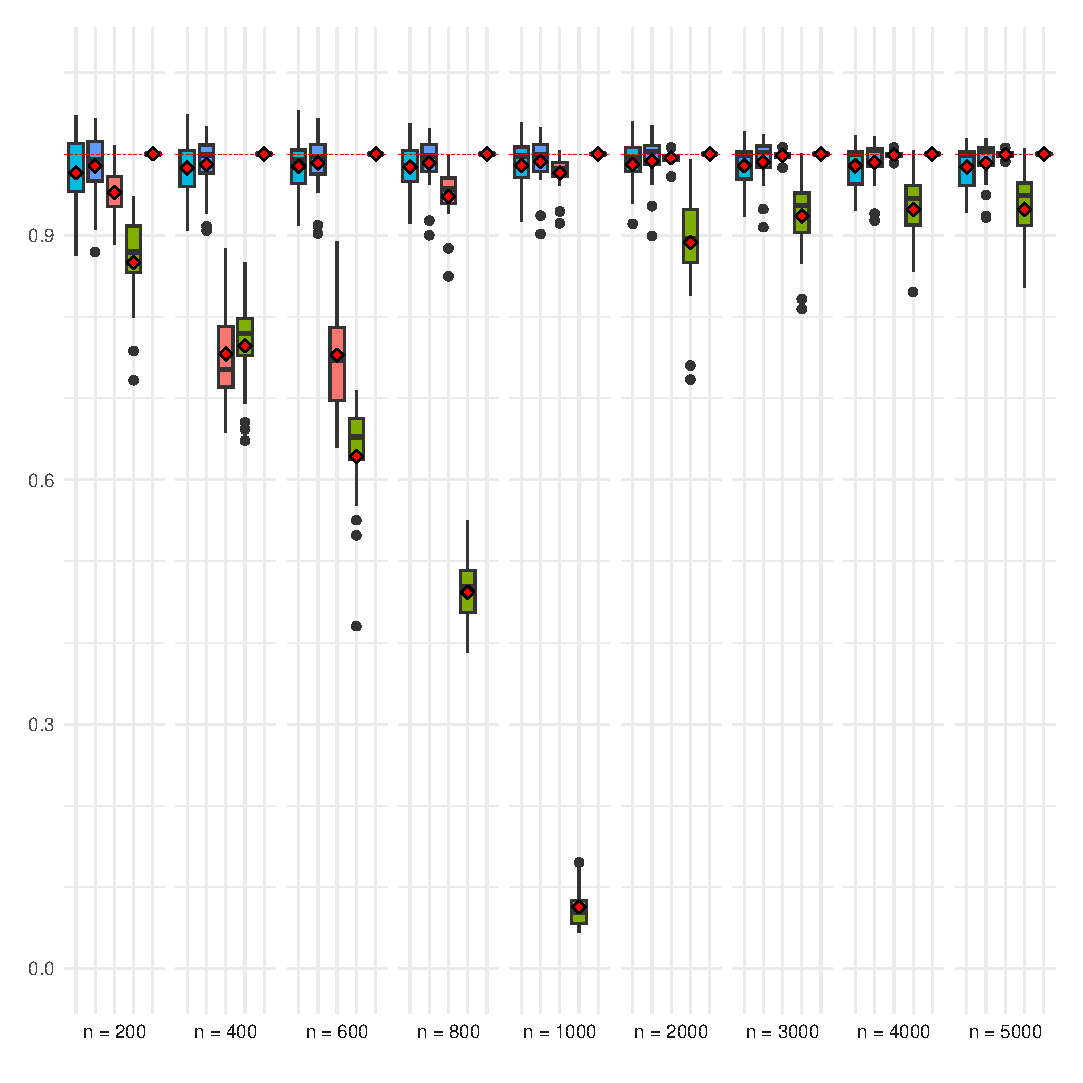
\includegraphics[width=6.01in,height=5in]
{graphs/weighted_rf_rmse_ratios_benchmarks_response}
\captionsetup{type=figure}
\captionof{figure}{Boxplots of RMSE ratios of HRF relative to WRF (cyan),
CRF (blue), Ridge (red), 2-Step Ridge (green), and HRF-MinVar (purple).
This is the counterpart to the manuscript's Figure~\ref{fig:win}, with
2-Step Ridge added; the wide range needed to accommodate the 2-Step Ridge
outliers compresses the detail among the remaining four benchmarks, which
is why the manuscript reports only this reduced set. For each
training-set size $n$, the boxplots are based on the 17 ratios
corresponding to the datasets listed in Table~\ref{table:datasets}.}
\label{fig:2step-ridge}
\end{center}

% -----------------------------------------------------------
\subsection*{Comment 2}
% -----------------------------------------------------------

\comment{Why not carrying out estimation on the same sample using a ridge
regression?  Again, helping the reader see the distinction and the merits
of one method over the other could be useful.}

\response
We have added a same-sample ridge regression benchmark (Ridge).
As with the second-sample variant, we impose the sum-to-one constraint and
select $\lambda$ by AIC.
Because the constraint is an equality, the standard ridge hat matrix must be
corrected; we derive the exact effective degrees of freedom analytically via
the economy SVD of the tree-prediction matrix.

The results are reported alongside the other benchmarks in Figure~\ref{fig:win}
(red boxplots) and in Appendix~\ref{sec:results-in-table-format}.
Ridge is a reasonably strong benchmark, but it is dominated by HRF, on
balance, at every training-set size.

% -----------------------------------------------------------
\subsection*{Comment 3}
% -----------------------------------------------------------

\comment{Why not focusing on variance minimisation, as for a minimum variance
portfolio?  Once the weights are derived this way and fixed, the bias, which
is a constant, could be removed in a second step, when forecasting.}

\response
We have implemented the minimum variance portfolio as an additional
benchmark, which we refer to as \textit{HRF-MinVar}.
The weights are obtained by minimising $\mathbf{w}^{\top}\widehat{\boldsymbol{\Sigma}}\mathbf{w}$
subject to $\mathbf{1}^{\top}\mathbf{w}=1$ and the leverage constraint
$\|\mathbf{w}\|_1\leq\kappa$.
The systematic bias of the combined predictor,
$\hat{b} = \mathbf{w}^{\top}\hat{\boldsymbol{\mu}}$ where $\hat{\boldsymbol{\mu}}$
denotes the vector of in-sample tree biases used in the HRF objective, is
then added back to each test-set forecast.
We compute this benchmark for both the sample and the shrunk
(Ledoit--Wolf nonlinear shrinkage) covariance estimator and for
$\kappa \in \{1, 2\}$, mirroring the HRF design; to keep the comparison
with HRF (shrinkage, $\kappa = 2$) as direct as possible, the main text
and tables report the matching HRF-MinVar (shrinkage, $\kappa = 2$)
variant.

The results are reported in Figure~\ref{fig:win} (purple boxplots) and in
Appendix~\ref{sec:results-in-table-format}, and are discussed in
Comment~4 below.

We would like to stress, however, that we still prefer to keep the bias
term $(w'\hat\mu)^2$ inside the joint optimization problem
\eqref{eq:mf1}--\eqref{eq:mf3}, rather than adopting the two-step
MinVar-plus-correction approach as our main method. The reason is that
the joint objective gives the weights themselves a chance to hedge
against bias: trees with a larger estimated bias are automatically
downweighted, in the same way that a mean-variance investor tilts a
portfolio away from assets with an unattractive risk-return trade-off.
The two-step approach, by contrast, fixes the weights on variance
grounds alone and can only correct the resulting aggregate bias
\emph{after the fact}, through a single constant shift; it cannot
differentially downweight the more biased trees. On our i.i.d.\ datasets, tree
biases turn out to be small and fairly homogeneous, so this distinction
happens not to matter much empirically, as the results below confirm.
But keeping the bias term in the objective is what gives HRF its
built-in insurance against bias in general, and, as we show in our
response to Comment~4 below, this insurance does come into play once we
move to the time-series application of Section~\ref{sec:fredmd}: there,
dropping the bias term from the optimization measurably erodes HRF's
advantage over RF. We would not want to give up this insurance merely
because it is not needed on the i.i.d.\ datasets studied here.

% -----------------------------------------------------------
\subsection*{Comment 4}
% -----------------------------------------------------------

\comment{Individual trees tend to have low bias but high variance, so the
variance component may dominate in practice.  This justifies the use of the
sample mean for the estimator of the bias of the individual trees, i.e.\ they
are small numbers close to zero dominated by the variance.  Would the
estimator perform the same or perhaps better if we just used a minimum
variance portfolio approach and forgot about the bias?}

\response
The empirical results for the HRF-MinVar benchmark described in Comment~3
provide a direct answer; see Figure~\ref{fig:win} and
Appendix~\ref{sec:results-in-table-format}.
HRF-MinVar (shrinkage, $\kappa = 2$) tracks HRF (shrinkage, $\kappa = 2$)
almost exactly, with RMSE ratios between $0.999$ and $1.001$ at every
training-set size, confirming the referee's intuition that the bias term in
the joint mean--variance objective contributes little in practice, at least
for i.i.d.\ data. 
Individual tree biases are indeed small relative to the variance, so the
HRF objective is effectively dominated by the variance component,
at least for i.i.d.\ data. 

This conclusion, however, is specific to the i.i.d.\ setting and does not
carry over to genuinely dependent, time-series data. The FRED-MD
financial-econometric application added in response to the Associate
Editor (Section~\ref{sec:fredmd}) gives us exactly such a testbed, since
there $\hat{\boldsymbol\mu}$ and $\hat{\boldsymbol\Sigma}$ are re-estimated
on a rolling basis from serially dependent tree residuals, rather than
computed once from a single i.i.d.\ training sample. Repeating the same
HRF-MinVar exercise for all 41 FRED-MD series (shrinkage, $\kappa = 2$,
$h = 1$) tells a different story: the mean RMSE ratio of HRF-MinVar
relative to RF is $1.007$, essentially wiping out HRF's mean RMSE ratio of
$0.982$ over the same series (Table~\ref{table:fredmd-summary}), and
HRF-MinVar improves on plain RF for only a handful of the 41 series,
compared to HRF's broad-based improvement. The gap between HRF and
HRF-MinVar is largest precisely in the credit/term-spread group, where
HRF's gains over RF are also largest. So for time-series data, unlike for
the i.i.d.\ datasets studied above, dropping the bias term from the
optimization is not innocuous: the rolling, time-varying tree biases are
apparently large and persistent enough, relative to the variance, that the
joint objective's automatic downweighting of biased trees actually earns
its keep.

This finding is informative in three directions.
First, it validates the HRF design on i.i.d.\ data: the method works well
even though the bias estimation step is noisy, because the variance
component is what matters there.
Second, it provides a useful robustness check for practitioners working
with i.i.d.\ data: a pure variance-minimization approach with a post-hoc
bias correction is equally effective and even simpler to implement in that
setting.
Third, and consistent with our response to Comment~3, it shows that this
simplification is not a free lunch in general: on time-series data the
bias term earns its place in the joint optimization problem
\eqref{eq:mf1}--\eqref{eq:mf3}, which is exactly why we keep it there as
our default design rather than adopting the two-step MinVar-plus-correction
approach.

% -----------------------------------------------------------
\subsection*{Comment 5}
% -----------------------------------------------------------

\comment{What is very interesting about negative weights is that they should
work better in situations where the trees are correlated.  From portfolio
optimisation theory we know that the weights will be all positive if the
correlations of the trees were small.  However, negative weights become more
likely as correlations increase.  Hence, the authors' method becomes even
more important and relevant when features are correlated, making tree
decorrelation more difficult.  I think remarking on the properties of
portfolio weights (especially in light of Point 4) as a function of
correlations would be relevant.}

\response
We thank the referee for this insightful observation, which we now make
explicit in the paper (Section~\ref*{sec:neg-weights}).

The connection follows directly from classical results in portfolio theory.
When the trees are mutually uncorrelated, the minimum-variance weights are
all positive: there is no benefit to short positions because each tree
contributes independent variance reduction. On the other hand,
if some pairwise tree correlations are non-zero,
the optimal portfolio can in principle reduce variance further by assigning negative weights to some trees (that is, short-selling trees). 
The leverage constraint $\|\mathbf{w}\|_1 \leq \kappa$ controls the degree
to which this is permitted: $\kappa = 1$ restricts weights to be non-negative
(no short-selling), whereas $\kappa = 2$ allows negative weights as long as they are not too large in (the sum of) absolute values. 

In the random forest setting this has a natural interpretation.
Trees are constructed to be decorrelated via feature subsampling
(the \texttt{mtry} parameter), but this decorrelation may be far from perfect when
the input features are themselves highly correlated.
In such datasets, trees may remain substantially correlated, and the gains
from $\kappa = 2$ over $\kappa = 1$ are expected to be largest.
Conversely, when features are nearly independent, and trees are already
well-decorrelated, $\kappa = 1$ generally suffices, and the additional flexibility from
$\kappa = 2$ adds little.
This provides a characterisation of when HRF with negative weights is most
valuable, and it is consistent with the empirical patterns we observe across
the benchmark datasets.
The corresponding passage has been added to Section~\ref*{sec:neg-weights}
of the revised manuscript.

% ============================================================
\section*{Additional Comments}
% ============================================================

% -----------------------------------------------------------
\subsection*{Additional Comment 1}
% -----------------------------------------------------------

\comment{It would be interesting to know whether one can learn something about
the methodology and the HRF estimator from the individual characteristics of
the datasets (e.g., variable correlations, fat-tailed data etc.).  For
instance, are there certain data features that systematically relate to larger
performance gains?}

\response
We investigated this question across the 17 datasets used in our study
(Table~\ref{table:datasets}). For each dataset we computed five
characteristics: the average pairwise absolute correlation among the
input features; the dispersion in the $p = 500$ individual trees' out-of-bag accuracy
$t\mbox{PE}_j$ (eq.~\eqref{eq:win0}, the same out-of-bag construction
used for the WRF benchmark), measured by its coefficient of variation
(CV), i.e.\ the ratio of the standard deviation to the mean of the
$p = 500$ values $t\mbox{PE}_1, \ldots, t\mbox{PE}_p$ within each
dataset, as a scale-free measure of how heterogeneous tree
\emph{quality} is within that dataset --- some trees may simply be
more accurate than others, and HRF can downweight the persistently
worse ones; the
excess kurtosis of the target variable, as a measure of fat-tailedness;
the number of features; and the ratio of the training-set size to the
number of features. We related each
characteristic (Spearman correlation) to HRF's performance gain, the
RMSE ratio of HRF relative to the equal-weighted RF, averaged across
\emph{all} training-set sizes $n \in \{200, \ldots, 5000\}$. $p$-values
are for a two-sided test of the null hypothesis that the corresponding
Spearman rank correlation is zero (\texttt{cor.test} in R), computed
exactly except for the number of features, which contains tied values
among the 17 datasets and for which the asymptotic $t$-approximation is
used instead.

\medskip
\begin{center}
\begin{tabular}{lcc}
\toprule
Characteristic & $\rho$ & $p$-value \\
\midrule
Feature correlation & $-0.07$ & $0.80$ \\
Tree-quality dispersion (CV = SD/mean of OOB tree $t\mbox{PE}_j$) & $-0.72$ & $0.002$ \\
Target kurtosis & $0.08$ & $0.76$ \\
Number of features $p$ & $0.05$ & $0.85$ \\
$n / p$ & $0.13$ & $0.61$ \\
\bottomrule
\end{tabular}
\end{center}
\medskip

Raw feature correlation and target kurtosis show essentially no
relationship with HRF's performance gain across our 17 datasets.
Dimensionality ($p$ and $n/p$) shows a weak, statistically insignificant
relationship.

The dispersion in individual-tree quality (Figure~\ref{fig:tree-quality})
is the only characteristic with a clear, statistically significant
relationship, and it is, as one might expect, \emph{negative}: datasets
in which some trees are persistently much worse than others show the
\emph{largest} gains from HRF over the equal-weighted forest. This is
consistent with your suspicion that HRF's ability to downweight
worse-performing trees is itself a source of its gains. For instance,
\textit{medical\_charges}, \textit{brazilian\_houses}, and \textit{pol}
have the most heterogeneous trees in our sample (coefficient of
variation $\approx 0.12$--$0.15$) and HRF/RF RMSE ratios as low as
$0.861$, whereas \textit{diamonds}, \textit{wine\_quality}, and
\textit{MiamiHousing2016} have the most homogeneous trees ($\approx
0.02$--$0.03$) and ratios close to one (0.97--1.02), averaged across all
training-set sizes.

\medskip
\begin{center}
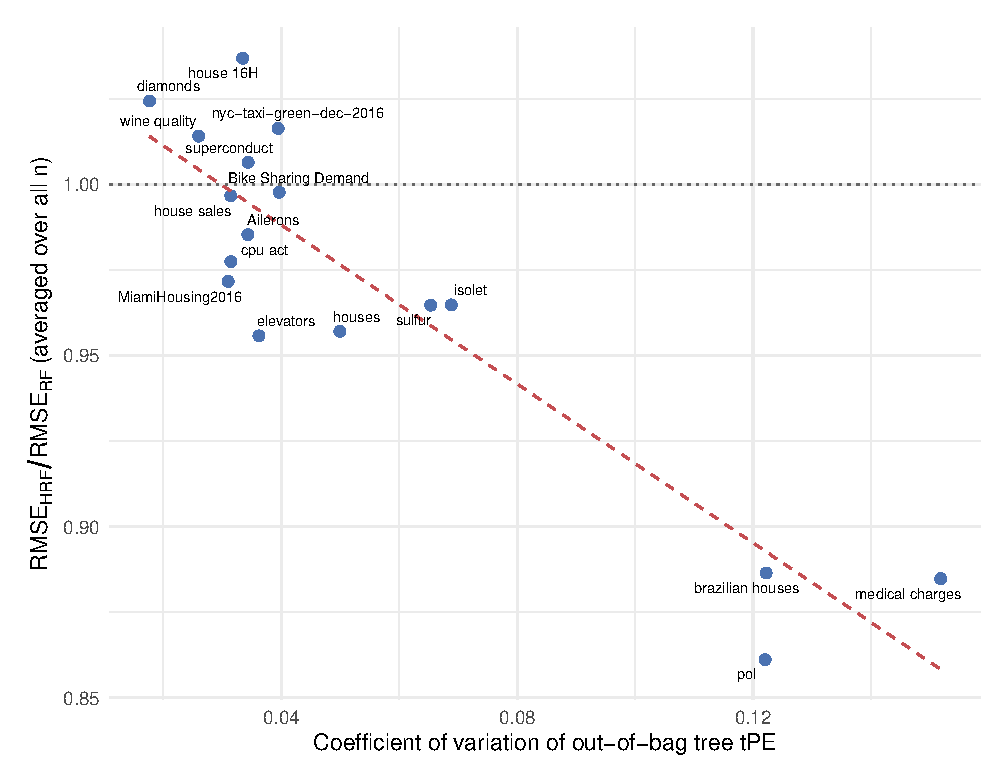
\includegraphics[width=5.5in]
{graphs/dataset_characteristics_tree_quality}
\captionsetup{type=figure}
\captionof{figure}{Coefficient of variation of out-of-bag tree accuracy
$t\mbox{PE}_j$ (horizontal axis) against the RMSE ratio of HRF
relative to the equal-weighted RF (vertical axis), averaged across all
training-set sizes $n \in \{200, \ldots, 5000\}$, for each of the 17
datasets. The dashed line is a simple linear fit.}
\label{fig:tree-quality}
\end{center}

We would like to flag this as a genuinely open finding rather than a
settled explanation. With only 17 datasets, and only one of five
characteristics tested reaching significance, we do not want to
over-interpret this correlation, and we have not incorporated it into
the manuscript. We report it here in the interest of full transparency;
a more systematic investigation of the relationship between tree quality
and the value of HRF (for example, using simulated data with a
controlled distribution of tree accuracy) would be a natural direction
for future work.

% -----------------------------------------------------------
\subsection*{Additional Comment 2}
% -----------------------------------------------------------

\comment{Many readers will naturally associate the leverage constraint with a
Lasso-type penalty and therefore expect a sparse solution, i.e.\ that only a
small number of trees receive nonzero weights.  However, the additional
portfolio equality constraint (i.e., the requirement that the weights sum to
one) changes the geometry of the optimisation problem, and often leads instead
to a dense weighting scheme.  It might be helpful to include a short remark
about this.}

\response
We have added Remark~\ref*{rem:dense} to Section~\ref*{sec:hrf} of the
revised manuscript.
[RESPONSE PENDING]


% -----------------------------------------------------------
\subsection*{Additional Comment 3}
% -----------------------------------------------------------

\comment{In section 3, the authors define their specific implementation of the
estimator: shrunk covariance matrix and a leverage constraint equal to 2.
Later in the paper, they compare results with a leverage constraint equal to
one and also compare to the estimator that uses the standard sample covariance
matrix.  A number of different intuitive notations are used to define these.
It would be ideal if this notation or some similar version could be used
everywhere.  Using shrinkage/sample and $\kappa$ (the leverage constraint)
equal to 1 or 2, everywhere is a possible solution.}

\response
We thank the referee for this suggestion.
We now state explicitly, in Section~\ref*{sec:hrf} right after HRF is
introduced, that from that point onward the term HRF refers by default to
our baseline specification, namely nonlinear shrinkage estimation of
$\Sigma$ combined with $\kappa = 2$, and that we flag explicitly any
instance in which we deviate from this default (for example, by using the
sample covariance matrix or a different value of $\kappa$), as we already
do throughout the paper whenever such comparisons are made.

% ============================================================
\bibliographystyle{apalike}
\bibliography{wolf}
% ============================================================

\end{document}
